\documentclass[12pt,oneside]{article}
\usepackage{light}
\newcommand{\mfigure}[3]{\bigskip\centerline{\resizebox{#1}{#2}{\includegraphics{#3}}}\bigskip}
\newcommand{\hint}[1]{({\it Hint: #1})}
\newcommand{\brule}[1]{\underline{\hspace{#1}}}
\newcommand{\ang}[1]{\left< #1 \right>}
\newcommand{\beats}{\rightarrow}

\newenvironment{falseproof}
{\begin{proof}[False proof]}
{\end{proof}}

\showsolutions
%\hidesolutions

\begin{document}
\generic{Quiz 2}{November 12, 2008}

\instatements{
\vspace{24pt}
\textbf{Name:} \rule{5in}{0.5pt}

\textbf{Circle the name of your recitation instructor}:

\begin{center}
\begin{tabular}{lllllll}
Bill & Brooke & Chieu & Jay & Ling & Nick & Spyros 
\end{tabular}
\end{center}

\begin{itemize}

\item This quiz is \textbf{closed book}, but you may have two $8.5
\times 11$'' sheet with notes in your own handwriting on both sides.

\item Calculators are not allowed.

\item You may assume all of the results presented in class.

\item Please show your work.  Partial credit cannot be given for a wrong
answer if your work isn't shown.

\item Write your solutions in the space provided.  If you
need more space, write on the back of the sheet containing the
problem.  Please keep your entire answer to a problem on that
problem's page.

\item Be neat and write legibly.  You will be graded not only on the
correctness of your answers, but also on the clarity with which you
express them.

\item If you get stuck on a problem, move on to others. The problems 
are not arranged in order of difficulty.

\item The exam ends at 9:30 PM.

\end{itemize}

%\vspace{0.25in}

\begin{center}
{\large
\begin{tabular}{|c|c|c|c|}
\hline
Problem & Points & Grade & Grader \\ \hline \hline
1 & 15 & & \\ \hline
2 & 10 & & \\ \hline
3 & 10 & & \\ \hline
4 & 10 & & \\ \hline
5 & 10 & & \\ \hline
6 & 10 & & \\ \hline
7 & 10 & & \\ \hline
8 & 10 & & \\ \hline
9 & 15 & & \\ \hline
Total & 100 & & \\ \hline
\end{tabular}
}
\end{center}
}
\instatements{\newpage}


% NOTES:
%
% Topics:
% - Sums and approximations
% - Recurrences
% - Counting methods
% - Repeat invariant problem of quiz 1
%
% Problems:
% SUMS AND ASYMPTOTICS
% + Asymptotic bounds (Fall06) change specific functions
% + Evaluating a sum (Fall06) using integral method
% + Evaluating a double sum by flipping sum
% RECURRENCES:
% + Regular divide and conquer recurrence via Akra-Bazzi (strong form needing to show h(x) - maybe logn?)
% - Regular homogenous linear recurrence
% + Prove Big O for a nonlinear recurrence via induction
% + Translate word problem into a nonhomogeneous recurrence
% COUNTING:
% + Regular counting problem (poker hands?)
% + Counting number of sequences that do not have certain subsequences
% + Combinatorial proof

%%%%%%%%%%%%%%%%%%%%%%%%%%%%%%%%%%%%%%%%%%%%%%%%%%%%%%%%%%%%%%%%%%%%%
% Asymptotics - Ling: these are new except for the n^n versus n! one, which I think is a nice one. I switched the order of that one though so that people cannot just memorize the answer.
%
\instatements{\newpage}
\begin{problem}{15} Circle every symbol on the left that could
correctly appear in the box to its right.  For each of the six
parts you may need to circle any number of symbols.

\begin{align*}
\mathbf{(a)} && O && \Omega && \Theta && o && \omega  && \sim && \hspace{1in} 
 6n^2+7n-10 && = \framebox[0.7in]{\insolutions{$O,\Omega,\Theta$}} & \left(n^2\right) \\[0.75in]
\mathbf{(b)} && O && \Omega && \Theta && o && \omega  && \sim && \hspace{1in} 
  6^n && = \framebox[0.7in]{\insolutions{$\Omega,\omega$}} & \left(n^6\right) \\[0.75in]
\mathbf{(c)} && O && \Omega && \Theta && o && \omega  && \sim && \hspace{1in} 
  n! && = \framebox[0.7in]{\insolutions{$O,o$}} & \left(n^n \right) \\[0.75in]
\mathbf{(d)} && O && \Omega && \Theta && o && \omega  && \sim && \hspace{1in} 
  \sum_{j=1}^{n} \frac{1}{j} && = \framebox[0.7in]{\insolutions{$O,\Omega,\Theta,\sim$}} & \left(\ln n \right) \\[0.75in]
\mathbf{(e)} && O && \Omega && \Theta && o && \omega  && \sim && \hspace{1in} 
  \ln(n^3) && = \framebox[0.7in]{\insolutions{$O,\Omega,\Theta$}} & \left(\ln n \right)
\end{align*}

\end{problem}

%%%%%%%%%%%%%%%%%%%%%%%%%%%%%%%%%%%%%%%%%%%%%%%%%%%%%%%%%%%%%%%%%%%%%
% Integral method
%
\newpage
\begin{problem}{10}
Give upper and lower bounds for the following expression which differ by at most 1.

% \hspace{0.5in} (\textit{Hint: $\frac{1}{(n+1)^2} \leq \frac{1}{n^2}$ for $n \geq 1$})

\[
\sum_{i=1}^{n} \frac{1}{i^3}
\]

\solution[\newpage]{
To find upper and lower bounds, we use the integral method:
\begin{align*}
\sum_{i=1}^{n} \frac{1}{i^3} & \leq 1+ \int_{1}^{n} \frac{1}{x^3} dx \\
& = 1 - \frac{1}{2}x^{-2} \Big |_{1}^{n} \\
& = 1 - \frac{1}{2}\left(\frac{1}{n^2} - 1\right) = \frac{3}{2} - \frac{1}{2n^2} \\
\sum_{i=1}^{n} \frac{1}{i^3} & \geq \frac{1}{n^3}+ \int_{1}^{n} \frac{1}{x^3} dx \\
& = \frac{1}{n^3}- \frac{1}{2}x^{-2}  \Big |_{1}^{n} \\
& = \frac{1}{n^3}- \frac{1}{2}\left(\frac{1}{n^2}-1\right) =  \frac{1}{2} + \frac{1}{n^3} - \frac{1}{2n^2}
\end{align*}
%
%Taking the difference between the upper and lower bounds we get:
%\[
%\left(\frac{3}{2} - \frac{1}{2n^2}\right) - \left(\frac{1}{2} + \frac{1}{n^3} - \frac{1}{2n^2}\right)
% = 1 - \left(\frac{1}{2n^2}+\frac{1}{n^3}\right)
%\]
%which is less than 1 for all n $\geq$ 1.
%
%We know that our bounds are within 1 of each other because:
%\begin{align*}
%upper - lower & = \left(\frac{n(n+1)}{2} + \frac{3}{2} - \frac{1}{2n^2}\right) - \left(\frac{n(n+1)}{2} + \frac{1}{n^3}+ \frac{1}{2} - \frac{1}{2n^2}\right) \\
%& = \left(\frac{3}{2} - \frac{1}{2}\right) -  \frac{1}{n^3}\\
%& = 1  - \frac{1}{n^3} \\
%& \leq 1.
%\end{align*}
%The last step comes about because $\frac{1}{(n+1)^2} \leq \frac{1}{n^2}$, so the second term is negative.
}

\end{problem}

%%%%%%%%%%%%%%%%%%%%%%%%%%%%%%%%%%%%%%%%%%%%%%%%%%%%%%%%%%%%%%%%%%%%%
% Double sum
%
%\instatements{\newpage}
%\begin{problem}{??}
%Find a closed form for the following summation:
%
%\[
%\sum_{x=0}^{n} \sum_{y=2}^{n} \frac{y^x (1-y)}{1-y^{n+1}}
%\]
%
%\solution[\vspace{3in}]{ Solution. }
%
%\end{problem}
%
%%%%%%%%%%%%%%%%%%%%%%%%%%%%%%%%%%%%%%%%%%%%%%%%%%%%%%%%%%%%%%%%%%%%%
% Akra-Bazzi
%

\insolutions{\vspace{0.3in}}
\begin{problem}{10}
Let $T(n)$ be a recurrence such that for all integers $n > 8$,

$$T(n) = 16T(\floor{n/2+\log{n}}) + n^{4}$$

Assume that $T(n) = 0$ for $n \leq 8$.  Find a $\Theta$ bound for $T(n)$.  Show your work.

\solution[\newpage]{Use Akra-Bazzi:
$a_1 = 16$, $b_1 = 1 / 2$, $h_1(n) = \floor{n/2+\log{n}} - n / 2$, $g(n) = n^4$, $p = 4$,
\[T(n) = \Theta \left( n^4 \left( 1 + \int_1^n \frac{u^{4}}{u^5} du \right) \right) =
\Theta \left( n^4 \left( 1 + \int_1^n \frac{1}{u} du \right) \right) = \Theta(n^4 \log n) \]
}

\end{problem}

%%%%%%%%%%%%%%%%%%%%%%%%%%%%%%%%%%%%%%%%%%%%%%%%%%%%%%%%%%%%%%%%%%%%%
% word problem
%

%\begin{problem}{10}
%A computer virus has been spreading. On the first day of its existence it spread to 100 computers.
%
%Word problem translated into non-homogeneous recurrence:
%We start with 5 flowers and zero seeds. Every day each subset of 5 flowers creates a seed. The day after the seed is created, it develops into a flower.
%
%\solution[\newpage]{ 
%$$T(n)=T(n-1)+{T(n-2) \choose 5}.$$
%}
%
%\end{problem}
\newpage
\begin{problem}{10}
At the end of year 0, Karen and Joe both have no money. In each subsequent year, the following happens:
\begin{enumerate}
\item On November 15th, Joe, an extremely good investor, has three times the amount of money he had at the beginning of the year.
\item On December 1st, Joe gives Karen the amount of money he had at the beginning of the year.
\item On December 15th, Karen makes \$10, which she promptly gives to Joe.
\end{enumerate}

Find a linear recurrence for the \textit{total} amount of money $T_n$ that the two have between them at the end of year $n$, including base cases. You do not have to solve the recurrence.

\vspace{0.3in}
You may choose to define recurrences, $K_n$ and $J_n$, for the amount of money that each of Karen and Joe have, respectively, but your final answer must be solely in terms of $T_n$.

(\textit{Hint: First find an expression for the amount of money Joe has at the end of year $n - 1$, $J_{n-1}$, in terms of $T_{n - 1}$ and $T_{n - 2}$.})

\solution[\newpage]{
At the end of year $n$, Karen has the amount she had at the end of year $n-1$, plus the amount that Joe had at the beginning of year $n$ (which is the same as the amount he had at the end of year $n-1$). Hence, $K_n = K_{n-1} + J_{n-1}$.

At the end of year $n$, Joe has three times the amount he had at the beginning of the year, minus the amount he had at the beginning of the year, plus the \$10 Karen gave him. Hence, $J_n = 3J_{n-1} - J_{n-1} + 10  = 2J_{n-1} + 10$.

\vspace{0.2in}
Now to determine the total that the two have, $T_n = K_n + J_n$. According to the hint, we rearrange the equation as $J_n = T_n - K_n$. Notice that $K_n = T_{n-1} = K_{n-1} + J_{n-1}$. Hence, we can substitute for $K_n$ to get the equation $J_n = T_n - T_{n-1}$.

\vspace{0.2in}
Finally, we substitute back into the equation for Joe to get:
\begin{align*}
J_n &= 2J_{n-1} + 10 \\
T_n - T_{n-1} &= 2(T_{n-1} - T_{n-2}) + 10 \\
T_n &= 3T_{n-1} - 2T_{n-2} + 10
\end{align*}

The base cases are $T_0 = 0$ and $T_1 = 10$.

Note that this is one possible recurrence for $T_n$; other equivalent recurrences are possible.

%During year $n - 1$, Karen and Joe earn $T_{n - 1} - T_{n - 2}$ between the two of them.  Of this amount, $T_{n - 1} - T_{n - 2} - 10$ was earned by Joe.  At the end of year $n - 1$, Joe has the amount he earned plus the \$10 Karen gave him, which is equal to $T_{n - 1} - T_{n - 2}$.  During year $n$, the two earn twice the amount of money Joe had at the beginning of the year plus \$10.  Thus, $T_n = T_{n - 1} + (2(T_{n - 1} - T_{n - 2}) + 10)$.  Simplifying, we have that $T_n = 3T_{n - 1} - 2T_{n - 2} + 10$.  The base cases are $T_0 = 0$ and $T_1 = 10$.
}
\end{problem}


%%%%%%%%%%%%%%%%%%%%%%%%%%%%%%%%%%%%%%%%%%%%%%%%%%%%%%%%%%%%%%%%%%%%%
% Induction O recurrence
%
\insolutions{\newpage}
\begin{problem}{10}
%Let $T(n)$ be defined by the recurrence
%$$ T(n)=3T(\lfloor n/2 \rfloor)^2$$
%for $n\geq 2$ with $T(1)=1$.
%Prove by induction that $T(n)=O(9^n)$.
%
%\solution[\vspace{3in}]{By induction. Prove $T(n)\leq c9^n$.
%Base case: $T(1)=1\leq 9c$ for $c\geq 1/9$. Inductive step: $T(n)=3T(\floor n/2\rfloor)^2\leq 3 c^2 9^{2\floor n/2\rfloor}\leq 3c^29^n\leq c9^n$ for $c\leq 1/3$. Take for example $c=1/9$.
%\bparts

%\ppart{10}
Let $T(n)$ be defined by the recurrence
$$ T(n)=2 \sqrt{T(n - 1)T(n - 2)}$$
for $n\geq 2$ with $T(0) = T(1) = 1$.  Prove by induction that
$T(n)=O(2^{2n / 3})$.

%(\textit{Hint: $2\cdot2^{2/3} > 3$.})

\solution[\newpage]{
\begin{proof}
Proof by strong induction.

Let $P(n)$ be the proposition that $T(n) \leq c2^{2n / 3}$, where $c$ is a very large constant, say $100$.

{\bf Base cases: } $T(0) = 1 \leq c$, $T(1)=1 \leq c 2^{2 / 3}$.

{\bf Inductive step: } Assume $P(k)$ for $0\leq k \leq n$ in order to prove $P(n+1)$. We derive
\begin{eqnarray*}
T(n+1) & = & 2 \sqrt{T(n)T(n - 1)} \\
& \leq & 2 \sqrt{c 2^{2n / 3}\cdot c 2^{2(n - 1) / 3}} \ \ \ \ \mbox{(By $P(n)$ and $P(n-1)$.)} \\
& = & c 2^{1 + (2n / 3 + 2n / 3 - 2 / 3) / 2} \\
& = & c 2^{2(n + 1) / 3}.
\end{eqnarray*}
This proves $P(n+1)$.
\end{proof}
}

%\ppart{5}
%Prove by induction that $T(n) = \Omega(2^{2n / 3})$.

%(\textit{Hint: $2^{2/3} < 3$.})

%\solution[\newpage]{
%\begin{proof}
%Proof by strong induction.  Let $P(n)$ be the proposition that $T(n) \geq c 2^{2n / 3}$, where $c = 1$.

%{\bf Base cases: } $T(0) = 1 \geq c$, $T(1)= 3 \geq c 2^{2 / 3}$.

%{\bf Inductive step: } Assume $P(k)$ for $0\leq k \leq n$ in order to prove $P(n+1)$. We derive
%\begin{eqnarray*}
%T(n+1) & = & 2 \sqrt{T(n)T(n - 1)} \\
%& \geq & 2 \sqrt{c 2^{2n / 3}\cdot c 2^{2(n - 1) / 3}} \ \ \ \ \mbox{(By $P(n)$ and $P(n-1)$.)} \\
%& = & c 2^{1 + (2n / 3 + 2n / 3 - 2 / 3) / 2} \\
%& = & c 2^{2(n + 1) / 3}.
%\end{eqnarray*}
%This proves $P(n+1)$.
%\end{proof}
%}

%\eparts

\end{problem}


%%%%%%%%%%%%%%%%%%%%%%%%%%%%%%%%%%%%%%%%%%%%%%%%%%%%%%%%%%%%%%%%%%%%%
% homogenous regular equation
%

\insolutions{\vspace{0.3in}}
\begin{problem}{10}
Solve the recurrence $T(n)=T(n-1)+12T(n-2)$ for $n\geq 2$ 
with $T(0)=2$ and $T(1)=1$.

\solution[\newpage]{
The characteristic polynomial is $x^2=x+12$ with solutions $x=4$ and $x=-3$.
This gives $T(n)=c_1 4^n+c_2 (-3)^n$ for $n\geq 0$.

Plugging in the base cases, we get the system of equations
\begin{align*}
2 &= c_1 + c_2 \\
1 &= 4c_1 - 3c_2
\end{align*}

Hence, $c_1 = c_2 = 1$, so $T(n)=4^n+(-3)^n$.
}

\end{problem}

%%%%%%%%%%%%%%%%%%%%%%%%%%%%%%%%%%%%%%%%%%%%%%%%%%%%%%%%%%%%%%%%%%%%%
% Counting problem (pigeonhole, substitution)
%
\insolutions{\newpage}
\begin{problem}{10}
%\bparts

%\ppart{5} Given a length $2n$ sequence of red and green balls, prove that if there are  $>n$ red balls, then there are at least 2 adjacent red balls.
%
%\solution[\vspace{3in}]{Let the red balls represent pigeons and let $\{1,2\}$, $\{3,4\}$, $\{5,6\}$, $\ldots$, $\{2n-1,2n\}$ represent holes. A red ball (pigeon) at position $i$  in the sequence of length $2n$ flies into the hole $\{2j-1,2j\}$ that contains $i$. By the pigeon hole principle, since there are more ($>n$) pigeons than holes ($=n$), there exists a hole, say $\{2j-1,2j\}$, that is occupied by at least two pigeons (red balls). This means that the two adjacent positions $2j-1$ and $2j$ are occupied by red balls. }
%
%\ppart{10}
How many length $2n$ sequences of red and green balls with exactly $m$ red balls satisfy the constraint that every red ball has a green ball adjacent to it on its left?  You may assume that $m \leq n$.  Express your answer using a single binomial coefficient; that is, using a single term of the form ${x \choose y}$.

\solution[\newpage]{Let $B$ be the set of length $2n$ sequences with $m$ red and $2n-m$ green balls such that every red ball has a green ball on its left. Let $A$ be the set of length $2n-m$ bit sequences with exactly $m$ ones and $2n-2m$ zeroes. Map a sequence from $A$ to a sequence in $B$ by mapping each 0 to a green ball and each 1 to a green ball followed by a red ball. This mapping is a bijection. By the bijection rule, $|B|=|A|={2n-m \choose m}$.  }

%\eparts
\end{problem}


%%%%%%%%%%%%%%%%%%%%%%%%%%%%%%%%%%%%%%%%%%%%%%%%%%%%%%%%%%%%%%%%%%%%%
% Combinatorial proof
%
\insolutions{\vspace{0.3in}}
\begin{problem}{10}

Find a combinatorial proof of the following identity by counting the number of pairs of sets $(X,Y)$ such that $X \subseteq Y \subseteq \set{1,2,\ldots,n}$ and $|Y| = m$:

\[
{n \choose m} 2^m = \sum_{i=0}^m {n \choose i} { n-i \choose m-i}
\]

\solution[\newpage]{ Let's consider each side of the equation.

\vspace{0.2in}
\textit{Looking at the left side:}

One way to count the number of pairs of sets $(X,Y)$ is to first count the number of possible sets $Y$, and then count the number of possible sets $X$ for each $Y$.

The number of sets $Y \subseteq \set{1,2,\ldots,n}$ with $|Y|=m$ is equal to ${n \choose m}$. For each $Y$, every value in $Y$ can either be in $X$ or not be in $X$. Since $|Y| = m$, the number of sets $X$ such that $X \subseteq Y$ is equal to the number of binary bit strings of length $m$, which equals $2^m$.

By the generalized product rule, the number of pairs of sets $(X,Y)$ such that $X \subseteq Y \subseteq \set{1,2,\ldots,n}$ and $|Y| = m$ is equal to ${n \choose m} 2^m$.

\vspace{0.2in}
\textit{Looking at the right side:}

Another way to count the number of pairs of sets $(X,Y)$ is to first count the number of possible sets $X$, and then count the number of possible sets $Y$ for each $X$.

Let $|X| = i$, where $i$ must range from 0 to m, since $X \subseteq Y$. For each value $i$, the number of sets $X \subseteq \set{1,2,\ldots,n}$ with $|X|=i$ is equal to ${n \choose i}$. For each $X$, we must pick the remaining $m-i$ elements from the remaining $n-i$ possible values to complete the set $Y$. Therefore, the number of sets $Y$ such that $X \subseteq Y$ is equal to ${n-i \choose m-i}$.

By the generalized product rule, the number of pairs of sets $(X,Y)$ such that $X \subseteq Y \subseteq \set{1,2,\ldots,n}$ and $|Y| = m$ is also equal to $ \sum_{i=0}^m {n \choose i} { n-i \choose m-i}$.

%For pairs of sets $(X,Y)$ such that $X \subseteq Y \subseteq \set{1,2,\ldots,n}$ and $|Y| = m$, the set $X$ has cardinality $0\leq |X|\leq m$. The number of sets $X\subseteq \set{1,2,\ldots,n}$ with cardinality $i$, $0\leq i\leq m$, is equal to ${n \choose i}$. A set $Y$ with $X \subseteq Y \subseteq \set{1,2,\ldots,n}$ and $|Y| = m$ consists of the $i$ elements of $X$ together with $m-i$ elements from the $n-i$ elements in $\set{1,2,\ldots,n}-X$. This means that there are ${n-i \choose m-i}$ sets $Y$ with $X \subseteq Y \subseteq \set{1,2,\ldots,n}$ and $|Y| = m$. By the generalized product rule, there are ${n \choose i} { n-i \choose m-i}$ pairs of sets $(X,Y)$ such that $|X|=i$, $X \subseteq Y \subseteq \set{1,2,\ldots,n}$, and $|Y| = m$. By the sum rule,  the number of pairs of sets $(X,Y)$ such that $X \subseteq Y \subseteq \set{1,2,\ldots,n}$ and $|Y| = m$ is equal to
  }

\end{problem}

%%%%%%%%%%%%%%%%%%%%%%%%%%%%%%%%%%%%%%%%%%%%%%%%%%%%%%%%%%%%%%%%%%%%%
% Counting problem
%
%\instatements{\newpage}
%\begin{problem}{1}
%The outcome of rolling a single dice is an integer in $\{1,2,3,4,5,6\}$.
%In how many ways can we roll 8 dice such that out of the 8 outcomes at least 4 are equal and such that the total number of different outcomes is exactly equal to 4.
%For example, we may roll a $1$ four times, a $2$ one time, a $3$ two times, and a $5$ one time; at least four of the outcomes are equal (to 1) and there are exactly four different outcomes ($1$, $2$, $3$, and $5$).
%
%Your answer may contain binomial coefficients, multiplications, and additions over integers.
%
%Explain your answer by defining a mapping and using the bijection rule or division rule.
%
%\solution{
%There are two kinds of 8 outcomes. The first kind has 4 equal outcomes, another 2 
%$$ 6\cdot 5\cdot {4 \choose 2} + 6\cdot {5 \choose 3}.$$
%}
%
%\end{problem}

\insolutions{\newpage}
\begin{problem}{15}

Your answers for the following questions may contain binomial coefficients of the form ${x \choose y}$, factorials, additions, multiplications, and divisions. Please explain your terms for partial credit.

\bparts
\ppart {5} How many 8-digit decimal sequences satisfy the following constraints?
\begin{enumerate}
\item Exactly four of the possible digits (the numbers from 0 to 9) appear.
\item One of the digits appears \textit{exactly} five times.
\end{enumerate}

For example, 01921111 is such a sequence.

\solution[\vspace{2.5in}]{
If one of the four digits appears \textit{exactly} five times, then each of the other three digits must appear only once each (such as in 11111234).  There are 10 choices for the repeated digit and ${9 \choose 3}$ choices for the remaining digits.  By the bookkeeper rule, these digits may be arranged in $\frac{8!}{5!1!1!1!}$ ways.  Thus, the number of such sequences is $10 {9 \choose 3} \frac{8!}{5!1!1!1!} = 282,240$.
}

\insolutions{\vspace{0.3in}}
\ppart {10} How many 8-digit decimal sequences satisfy the following constraints?
\begin{enumerate}
\item Exactly four of the possible digits appear.
\item One of the digits appears \textit{at least} four times.
\end{enumerate}

For example, 01921111 and 01921112 are both such sequences.

\solution[\newpage]{
If one of the four digits apears \textit{at least} four times, then it must be the case that either one digit appears five times as in the previous part, \textit{or} one digit appears exactly four times, a second digit appears exactly twice, and each of the other two digits appears only once each (such as in 11112234).

In the new case, there are 10 choices for the digit that appears four times, 9 remaining choices for the digit that appears twice, and ${8 \choose 2}$ remaining choices for the other digits.  By the bookkeeper rule, these digits may be arranged in $\frac{8!}{4!2!1!1!}$ ways.  Thus, there are $10 \cdot 9 \cdot {8 \choose 2} \frac{8!}{4!2!1!1!}$ such sequences.

Therefore, the total number of sequences is the sum of the two disjoint sets, which equals $10 \cdot 9 \cdot {8 \choose 2} \frac{8!}{4!2!1!1!} + 10 {9 \choose 3} \frac{8!}{5!1!1!1!} = 2,399,040$.
}
\eparts

\end{problem}


\end{document}


%%%%%%%%%%%%%%%%%%%%%%%%%%%%%%%%%%%%%%%%

\begin{problem}{10} 
In how many ways

A letter-digit combination is a pair $(l,d)$ with $l$ a letter in the alphabet $\{A,B,C,\ldots, Z\}$ and $d$ a digit in the set of numbers $\{0,1,2,\ldots, 9\}$. 

Count the number of sets of letter-digit combinations of size 4 that contain 
\begin{itemize}
\item two letter-digit combinations $(l,d)$ and $(l',d')$ with $l=l'$, $d\leq 5$ and $d'\leq  5$, and
\item two letter-digit combinations $(l,d)$ and $(l',d')$ with $l=l'$, $d> 5$ and $d'>5$.
\end{itemize}
For example, 
$$\{ (A,1), (A,3), (D,9), (D,6)\}$$
and
$$\{ (A,1), (A,3), (A,7), (A,8)\}.$$

Explain your answer by defining a mapping and using the bijection rule or division rule.

\solution{
$$ 26\cdot {6 \choose 2} \cdot 26 \cdot {4 \choose 2}.$$
}

\end{problem}


%%%%%%%%%%%%%%%%%%%%%%%%%%%%%%%%%%%%%%%%%%%%%%%%%%%%%%%%%%%%%%%%%%%%%
% SAME PROBLEM AS QUIZ 1 - but we will change from rotating 4 tiles to rotating 5 tiles 
%
\instatements{\newpage}
\begin{problem}{??}\label{slipped_disc}
SAME PROBLEM AS QUIZ 1 - but we will change from rotating 4 tiles to rotating 5 tiles 

The Slipped Disc Puzzle\texttrademark\ consists of a track holding 9 
circular tiles. In the middle is a disc that can slide left and right and rotate 
$180\,^{\circ}$
to change the positions of \emph{exactly} four tiles. As shown below, there are 
three ways to manipulate the puzzle:

\begin{description}
\item[Shift Right:] The center disc is moved one unit to the right (if there is space)
\item[Rotate Disc:] The four tiles in the center disc are reversed
\item[Shift Left:] The center disc is moved one unit to the left (if there is space)
\end{description} 

\begin{center}
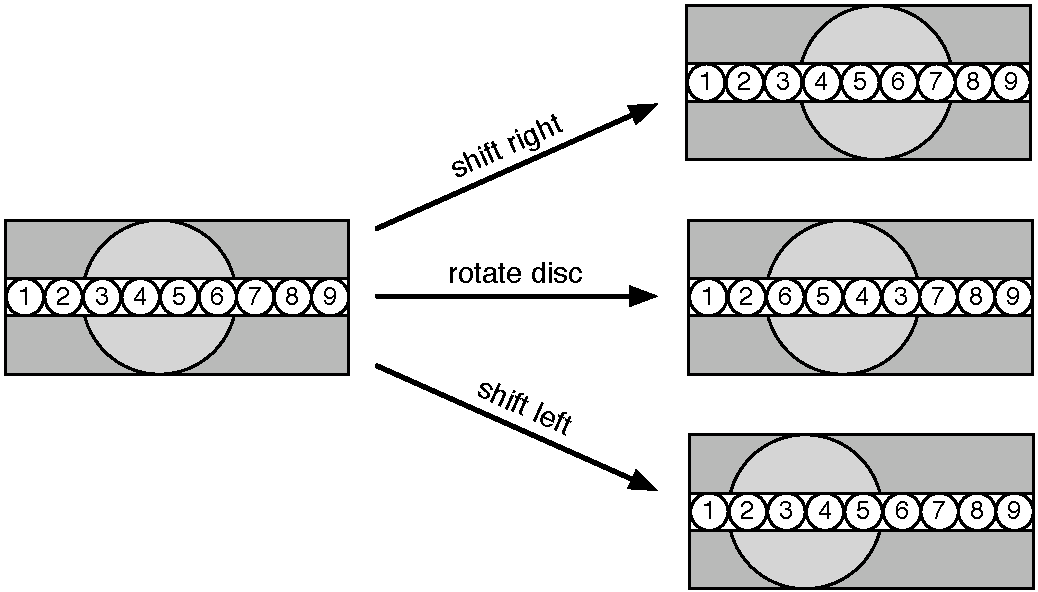
\includegraphics[width=5in]{1d-puzzle-transitions}
\end{center}

Prove that if the puzzle starts in an initial state with all but tiles 1 
and 2 in their natural order, then it is impossible to reach a goal state 
where all the tiles are in their natural order.  The initial and goal states are shown below:

\begin{center}
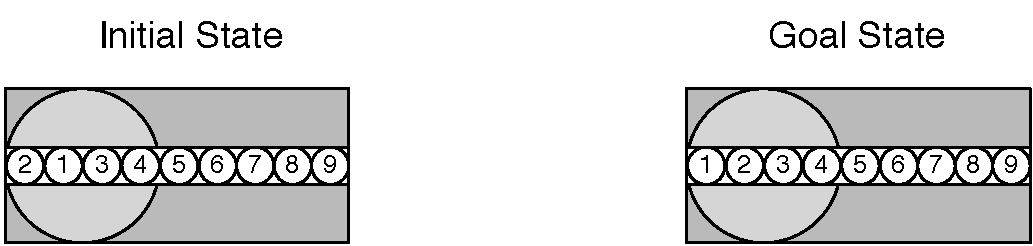
\includegraphics[width=5in]{1d-puzzle-challenge}
\end{center}

Write your proof on the next page...

\solution[\newpage]{
Order the tiles from left to right in the puzzle. Define an \emph{inversion} to be a pair of tiles that is out of their natural order (e.g. 4 appearing to the left of 3). 
\begin{lemma*}
Starting from the initial state there is an odd number of inversions after any number of transitions.
\end{lemma*}
\begin{proof}
The proof is by induction.  Let $P(n)$ be the proposition that starting from the initial state there is an odd number of inversions after $n$ transitions.

{\bf Base case:} After 0 transitions, there is one inversion, so $P(0)$ 
holds.

{\bf Inductive step:} Assume $P(n)$ is true.  Say we have a configuration 
that is reachable after $n + 1$ transitions.
\begin{enumerate}
\item Case 1: The last transition was a shift left or shift right

In this case, the left-to-right order of the discs does not change and thus the number of inversions remains the same as in 

\item The last transition was a rotate disc.

In this case, six pairs of disks switch order.  If there were $x$ inversions among these pairs after $n$ transitions, there will be $6 - x$ inversions after the reversal. If $x$ is odd, $6-x$ is odd, so after $n+1$ transitions the number of inversions is odd.
\end{enumerate}
\end{proof}

Conclusion: Since all reachable states have an odd number of inversions and the goal state has an even number of inversions (specifically 0), the goal state cannot be reached.
}

\instatements{
\newpage
{\bf room for problem \ref{slipped_disc}...}
}

\end{problem}
